%\section{Une section}

% remarque : pour qu'un mot se retrouve dans le lexique : \MotDefinition{asymptote horizontale}{} 

\begin{aconnaitre}
Une \MotDefinition{translation}{} consiste à faire glisser une figure selon un \MotDefinition{vecteur}{} donné.\\[0.5em]
\begin{minipage}[c]{0.58\linewidth}
Un \textbf{vecteur} est donné par :
\begin{itemize}
 \item une direction (c'est la direction de la droite)
 \item un sens (c'est le sens de la flèche)
 \item une longueur (c'est la longueur du segment)
 \end{itemize}
 \end{minipage} \hfill%
 \begin{minipage}[c]{0.38\linewidth}
 \begin{center} 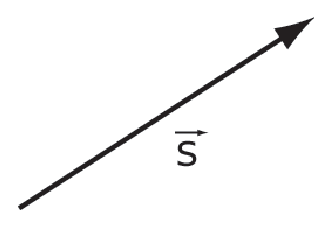
\includegraphics[width=2.3cm]{vecS} \end{center}
 \end{minipage} \\
\end{aconnaitre}

\begin{methode*1}[La translation]

 \begin{exemple*1}
Construis l'image du triangle $ABC$ par la translation de vecteur $\vec{a}$ :
%\begin{tabularx}{\linewidth}{X|X|X}
%\textcolor{H1}{$\circled{1}$} & \textcolor{H1}{$\circled{2}$} & \textcolor{H1}{$\circled{3}$} \\
%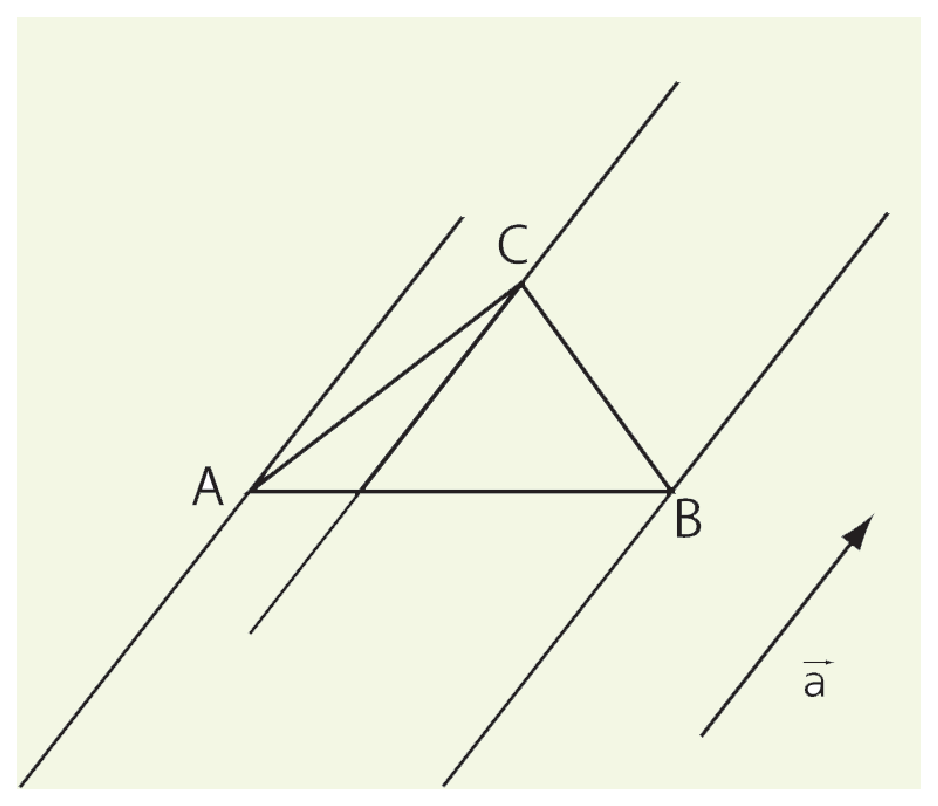
\includegraphics[width=4.3cm]{triangleABC_vecA1} & 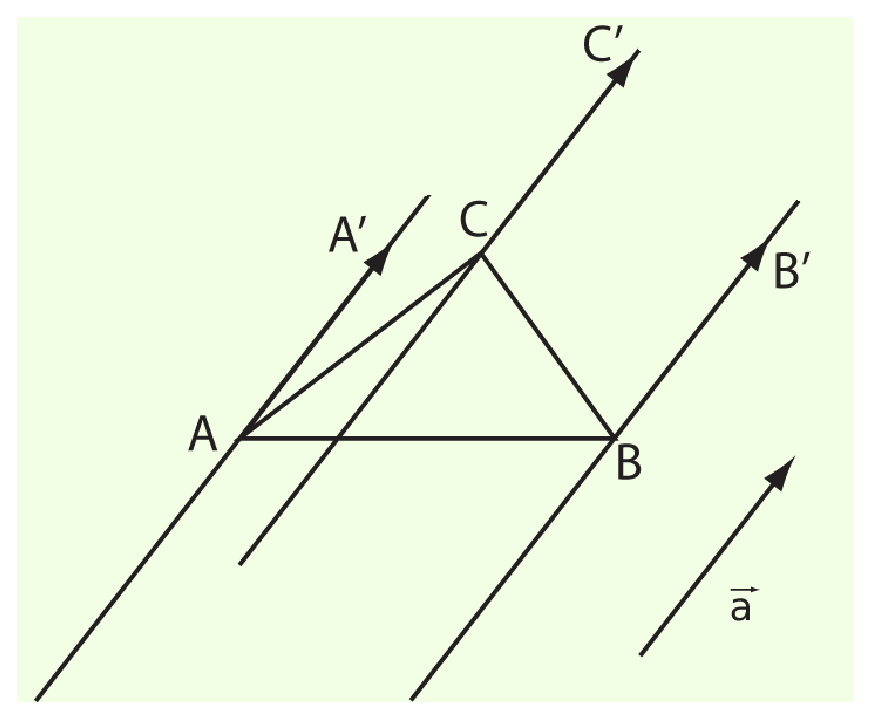
\includegraphics[width=4.3cm]{triangleABC_vecA2} & 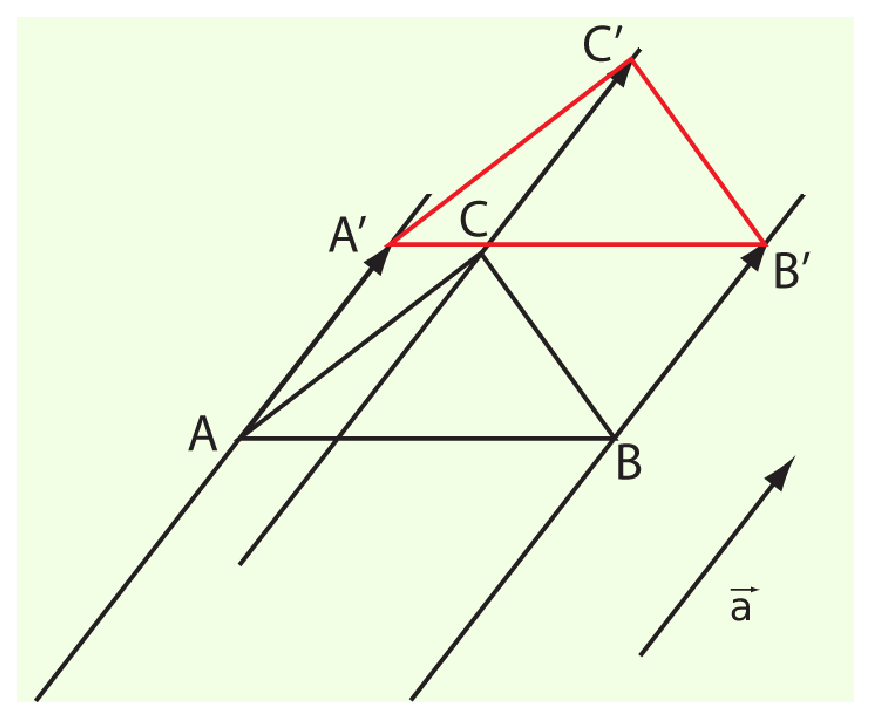
\includegraphics[width=4.3cm]{triangleABC_vecA3} \\
%\end{tabularx} \\
%\textcolor{H1}{$\circled{1}$} On trace des droites parallèles au vecteur $\vec{a}$ passant par les sommets de la figure ;
%\textcolor{H1}{$\circled{2}$} On reporte sur les droites le vecteur $\vec{a}$ en respectant le sens donné par la flèche ;
%\textcolor{H1}{$\circled{3}$} On relie les sommets entre eux.
 \end{exemple*1}
 
 \begin{exemple*1}
$A'$ est l'image de $A$ par une translation. Construis l'image $B'$ de $B$ par cette translation :
%\begin{tabularx}{\linewidth}{X|X}
 %\textcolor{H1}{$\circled{1}$} & \textcolor{H1}{$\circled{2}$} \\
% 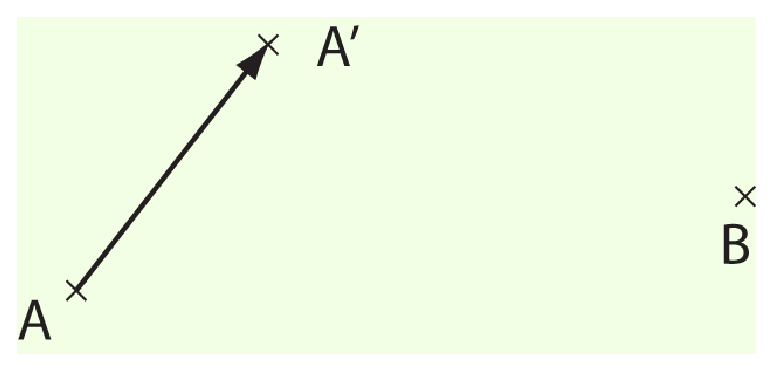
\includegraphics[width=5.5cm]{translationAAB} &  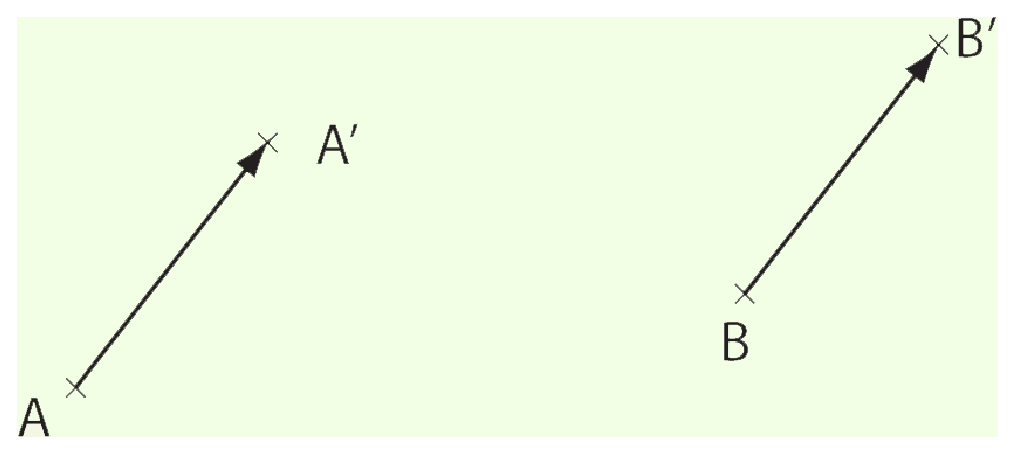
\includegraphics[width=7cm]{translationAABB} \\ 
%\end{tabularx} \\
%\textcolor{H1}{$\circled{1}$} On trace le vecteur $\vec{AA'}$ ;
%\textcolor{H1}{$\circled{2}$} On construis l'image du point $B$ par la translation de vecteur $\vec{AA'}$.
 \end{exemple*1}

 \exercice
En t'aidant du quadrillage de ton cahier, reproduis puis construis l'image de la figure par la translation de vecteur $\vec{b}$ :
\begin{center} \includegraphics[width=5.7cm]{quadrillage_vecB} \end{center}
%\correction

 \end{methode*1}
 
%%%%%%%%%%%%%%%%%%%%%%%%%%%%%%%%%%%%%%%%%%%%%%%%%%%%%%%%%%%%%%%%%%%%%%%

\begin{aconnaitre}
Une \MotDefinition{rotation}{} est définie par son \textbf{centre} et son \textbf{angle}.

L'angle de rotation est \textbf{positif} si la rotation s'effectue dans le sens contraire des aiguilles d'une montre et \textbf{négatif} sinon.
\end{aconnaitre}

\begin{remarque}
La rotation de centre $O$ et d'angle $\alpha$ est notée : $R(O ; \alpha)$.
 \end{remarque}

\begin{methode*1}[La rotation]

 \begin{exemple*1}
 Construis l'image du triangle $ABC$ par la rotation $R(O ; - 45^\circ)$ :
 
%\begin{tabularx}{\linewidth}{X|X}
 %\textcolor{H1}{$\circled{1}$} & \textcolor{H1}{$\circled{2}$} \\
%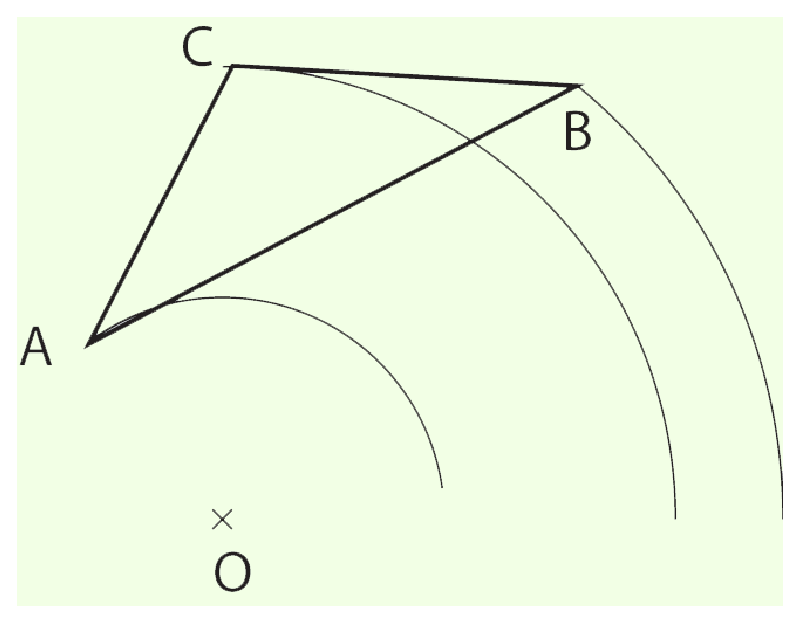
\includegraphics[width=4.7cm]{rotation_triangleABC} &  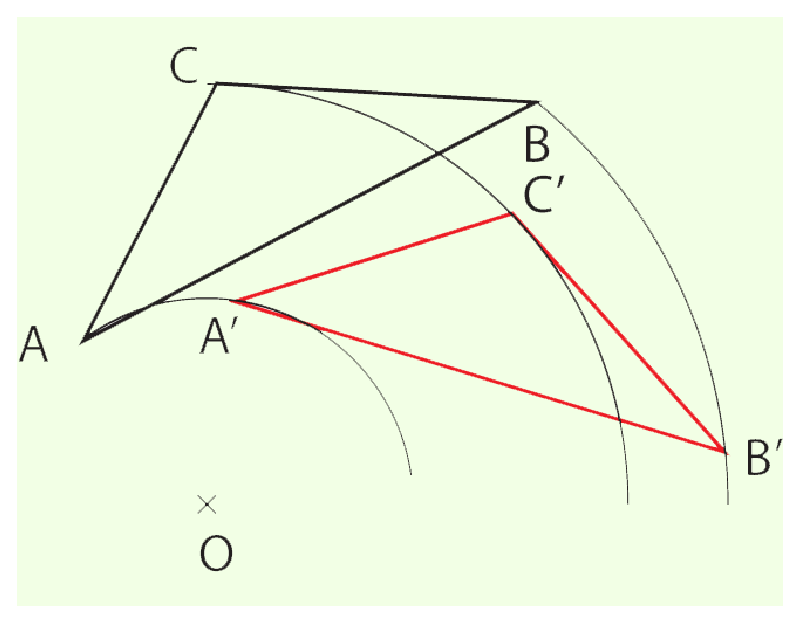
\includegraphics[width=4.7cm]{rotation_triangleABC2} \\ 
%\end{tabularx} \\

\textcolor{H1}{$\circled{1}$} La rotation s'effectue dans le sens des aiguilles d'une montre. On trace des arcs de cercles de centre $O$ passant par les sommets $A$, $B$ et $C$ ;
\textcolor{H1}{$\circled{2}$} On reporte l'angle de rotation sur tous les arcs de cercles ($\widehat{AOA'} = 45^\circ$) et on relie les sommets entre eux.
 \end{exemple*1}
 
\begin{exemple*1}
$A'$ et $B'$ sont l'image de $A$ et $B$ par une rotation. Détermine le centre de la rotation ainsi que l'angle de rotation :

\begin{minipage}[c]{0.44\linewidth}
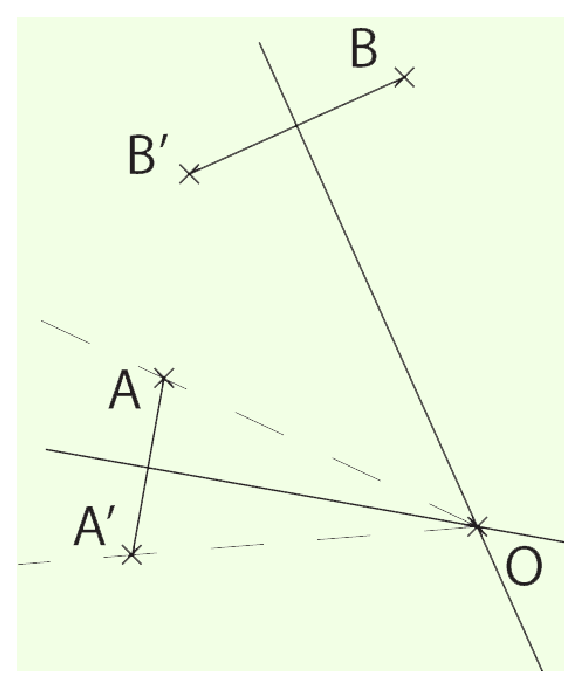
\includegraphics[width=3.7cm]{centre_rotation}
 \end{minipage} \hfill%
 \begin{minipage}[c]{0.52\linewidth}
On trace les médiatrices de $[AA']$ et $[BB']$. L'intersection des médiatrices donne le centre de la rotation $O$. \\[0.5em]
La rotation s'effectue dans le sens inverse des aiguilles d'une montre alors l'angle est positif. L'angle $\widehat{AOA'} = 30^\circ$ donc l'angle de rotation est $+ 30^\circ$
 \end{minipage} \\ 
 \end{exemple*1}

 \exercice
 En t'aidant du quadrillage de ton cahier, reproduis puis construis l'image de la figure par la rotation $R(O ; 60^\circ)$ : \\[0.5em]
 \begin{center} 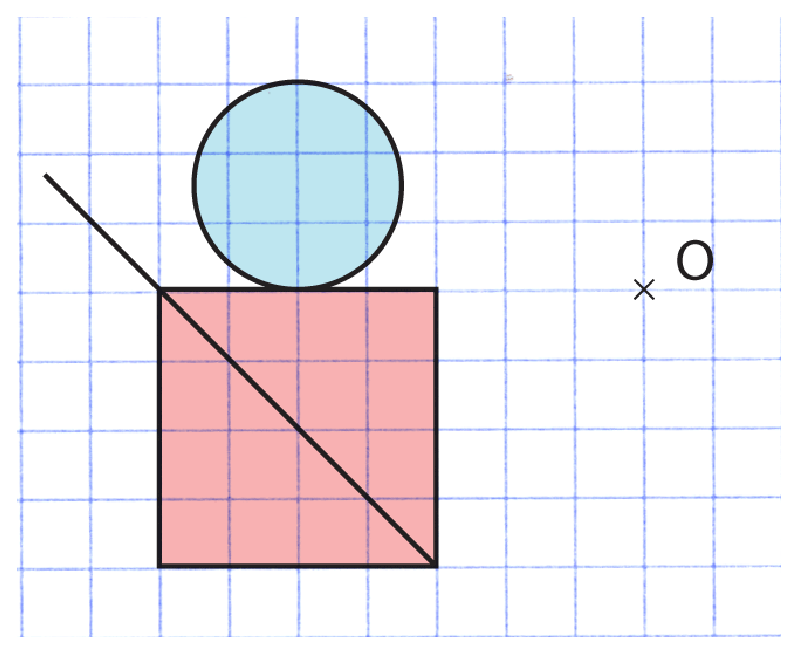
\includegraphics[width=5.2cm]{rotation_O60} \end{center}
%\correction

 \end{methode*1}
 
%%%%%%%%%%%%%%%%%%%%%%%%%%%%%%%%%%%%%%%%%%%%%%%%%%%%%%%%%%%%%%%%%%%%%%%
